\section{Technical Part}
% Sec 3.1: Technical part: Summary of the technical solution
% Sec 3.2: Technical part: Details of the technical solution; you may want to decompose this section into several subsections; add figures to help your explanation.


\begin{figure*}[t]
    \centering
    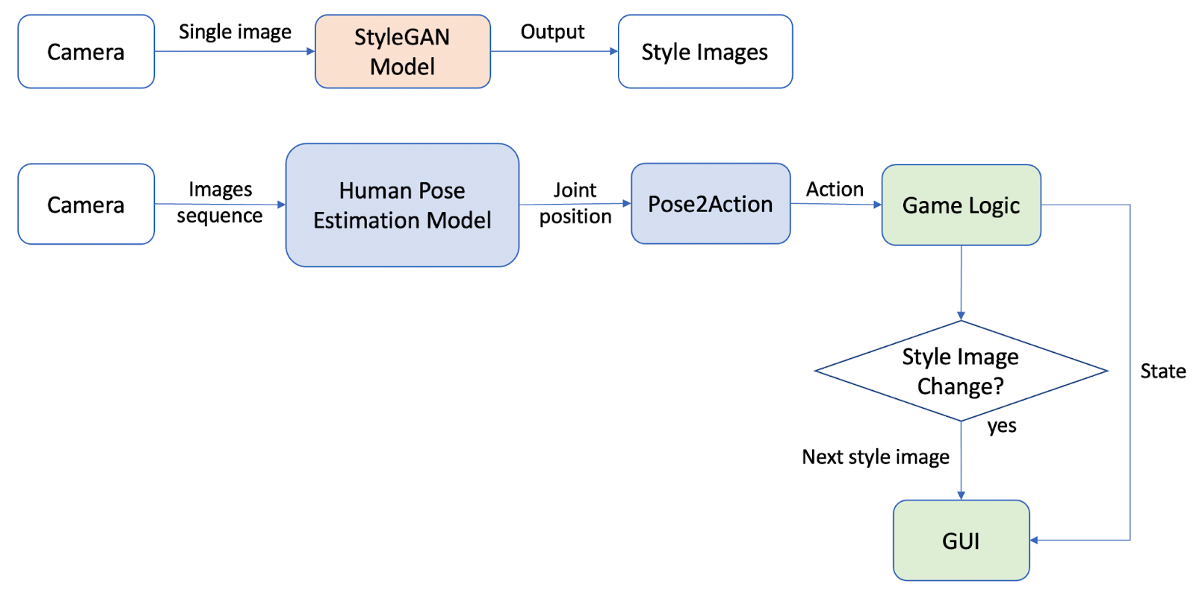
\includegraphics[scale=.4]{fig/flow.png}
    \caption{System flow chart. Players will take a selfie respectively as their player avatar before the game starts. During the game, the camera will capture the players’ human pose, reflecting the human pose in the game. The faces in the game will also change by time according to the health points of each player.}
    \label{fig:flow}

\end{figure*}

Figure \ref{fig:flow} shows the flow chart of our game. We'll introduce \textbf{styleGAN}, \textbf{human pose estimation} and \textbf{game interface} in this section.

%-------------------------------------------------------------------------
\subsection{StyleGAN}
In order to mix the style of two real faces, we utilize the style encoding\cite{richardson2021encoding}, style mixing, latent code interpolation and StyleGAN\cite{karras2019style} \cite{karras2020analyzing} inference. Firstly, Style encoding aims to find a corresponding latent code $w$ from a real image $I$ such that the generated image $I'$ from $w$ is very similar to the original real image $I$ (you can regard this task as a reconstruction task). We use Style encoding to transform source images $I_{source}$ and target image $I_{source}$ to obtain corresponding latent vectors $w_{source}$ and $w_{target}$ and then use these latent vectors to do latent code interpolation.


Secondly, the main idea of latent code interpolation is to get a sequence of latent codes $[w_1,...,w_n]$ by interpolating different proportion of latent code $w_{source}$ and $w_{target}$, where $n$ is the length of sequence (e.g. $w_1$ consists of 95\% of $w_{source}$ and 5\% of $w_{target}$ ; $w_2$ consists of 90\% of $w_{source}$ and 10\% of $w_{target}$...)

Finally, we will put results from latent code interpolation $[w_1,...,w_n]$ into StyleGAN model and the model outputs a sequence of images $[I_1,...,I_n]$ that mixed the style of $w_{source}$ and $w_{target}$. From the left part of the sequence $I_1,I_2,...$ preserves more information of $w_{source}$ while the right part of the sequence $I_n,I_{n-1},...$ preserves more information of $w_{target}$. In our game, we will change the player's face base on image sequences $[I_{source},I_1,I_2, ... ,I_n,I_{target}]$ whenever the player loses health points. 

\subsection{Human pose estimation}
as shown in Figure~\ref{fig:medpose}
\begin{figure}[h]
    \begin{center}
        \includegraphics[width=1.0\linewidth]{fig/medpose.png}
    \end{center}
    \caption{\textbf{33 key points predicted}
    }
    \label{fig:medpose}
\end{figure}

In order to reflect the human action in the game, we need a model that can predict real-time human pose. Besides, due to the immediacy we require in our game and the laptop we use without the high Compute Capability GPU, the model cannot be too computationally expensive. Therefore, we discard some state-of-the-art human pose estimation frameworks such as YOLOv7\cite{Alpher06}. 

Instead, we select \textbf{mediapipe}\cite{med} developed by \textbf{Google} to achieve real-time human pose estimation. It captures the real-time image from the camera and performs real-time single person human pose estimation, which can predict 33 key points as Figure \ref{fig:medpose} shows.

In order to predict two people's key points in one image, we crop the image into two halves. One person stands on the left side and the other stands on the right side. We perform their pose estimation individually. The position matrix of the left-side person is denoted as $M_{left}=[[x_1, y_1],[x_2, y_2],...,[x_{33}, y_{33}]]$ and the position matrix of the right-side person is denoted as $M_{right}=[[x_1, y_1],[x_2, y_2],...,[x_{33}, y_{33}]]$, where $x$ and $y$ are the positions of each key point. We can use these 33 key points to predict actions such as "raise right hand." Take "raising right hand" for example. When the position $y$ of key point 15, the right wrist, is larger than the position $y$ of key point 0, the nose, we can define the action as "raising right hand." This is how the pose-to-action step work.


\begin{figure}[ht]
    \centering
    \includegraphics[scale=.3]{medpose.png}
    \caption{33 key points predicted by mediapipe.}
    \label{fig:medpose}
\end{figure}


%-------------------------------------------------------------------------
\subsection{Game interface}

In this part, we will need to create the GUI of this game. At the beginning of the game, two players will first take a selfie through the camera, and the pictures will become the faces of the characters in the game and show on the screen. Next, when the game starts, we will receive the real-time actions from the previous part of human pose estimation (Sec. 2.2), then the game characters will do the corresponding actions on the screen.

Throughout this game, whenever the character is attacked, his/her health point will drop. Meanwhile, we will switch his/her face to the next image which comes from the sequence of the player's style images (Sec. 2.1). The game will come to the end if one of the character's face completely become the pre-selected target image, in another words, the health point equals to zero.